\documentclass[conference]{IEEEtran}
\IEEEoverridecommandlockouts
\usepackage[utf8]{inputenc}
\usepackage[T1]{fontenc}
\usepackage[spanish,es-tabla]{babel}
\usepackage{cite}
\usepackage{amsmath,amssymb,amsfonts}
\usepackage{algorithmic}
\usepackage{graphicx}
\usepackage{textcomp}
\usepackage{xcolor}
\usepackage{booktabs}
\usepackage{array}
\usepackage{tabularx}
\usepackage{microtype}

\makeatletter
\def\section{\@startsection{section}{1}{\z@}{1.3ex plus 0.8ex minus 0.2ex}%
{0.5ex plus 0.4ex minus 0.1ex}{\normalfont\normalsize\bfseries\scshape\centering}}
\def\subsection{\@startsection{subsection}{2}{\z@}{1.0ex plus 0.6ex minus 0.2ex}%
{0.4ex plus 0.3ex minus 0.1ex}{\normalfont\normalsize\bfseries\itshape}}
\makeatother

\def\BibTeX{{\rm B\kern-.05em{\sc i\kern-.025em b}\kern-.08em
    T\kern-.1667em\lower.7ex\hbox{E}\kern-.125emX}}

\begin{document}

\title{Predicción de la desviación temporal del transporte público de Cusco mediante aprendizaje automático\\
\large Entregable 2: Implementación y Evaluación Experimental
\thanks{Trabajo del curso 1INF02 Aprendizaje de Máquina (horario H-1081), semestre 2026-2. Docentes: Dr. Edwin Alvarez Mamani y Dr. César Armando Beltrán Castañón.}
}

\author{
\IEEEauthorblockN{Italo Marcelo Carrion Segura}
\IEEEauthorblockA{\textit{Facultad de Ciencias e Ingeniería} \\
\textit{Pontificia Universidad Católica} \\
\textit{del Perú} \\
Lima, Perú}
\and
\IEEEauthorblockN{Mauricio Lucio Arenales Aquino}
\IEEEauthorblockA{\textit{Facultad de Ciencias e Ingeniería} \\
\textit{Pontificia Universidad Católica} \\
\textit{del Perú} \\
Lima, Perú\\[1.8ex]
\IEEEauthorblockN{Italo Mijail Ramos Diaz}
\IEEEauthorblockA{\textit{Facultad de Ciencias e Ingeniería} \\
\textit{Pontificia Universidad Católica} \\
\textit{del Perú} \\
Lima, Perú}}
\and
\IEEEauthorblockN{Alvaro Erlin Pesantes Advincula}
\IEEEauthorblockA{\textit{Facultad de Ciencias e Ingeniería} \\
\textit{Pontificia Universidad Católica} \\
\textit{del Perú} \\
Lima, Perú}
}

\maketitle

\begin{abstract}
La puntualidad y la predictibilidad de los tiempos de recorrido son centrales para la calidad del transporte público urbano, pero en Cusco la variabilidad de cada vuelta dificulta la planificación y el control operativo. Este trabajo desarrolla, audita y valida un marco experimental riguroso y reproducible de Machine Learning supervisado para predecir la desviación temporal respecto al horario programado (\textit{difference\_time}) en cada punto de control del recorrido, utilizando exclusivamente información previa. A partir de dos conjuntos de datos del Sistema de Transporte Inteligente local (Times.csv, con 4\,707 vueltas expandidas a 84\,726 registros, y Monitoring.csv, con 1.63 millones de registros GPS), se implementó una partición cronológica estricta por semanas (entrenamiento: 6--19 de enero; validación: 20--26 de enero; prueba: 27 de enero--1 de febrero de 2025). Se compararon modelos de referencia (cero, promedio histórico, persistencia estricta y persistencia de último valor) con regresión lineal regularizada (Ridge, Lasso), redes neuronales (MLP con decaimiento $L_2$ y parada temprana) y ensambles (Random Forest, HistGradientBoosting, XGBoost y LightGBM con pérdida $L_1$). Una auditoría semántica demostró que \textit{difference\_time} coincide en el 100.0\,\% de las observaciones válidas con el truncamiento entero de la desviación horaria en minutos. La selección de características con Boruta redujo el espacio de 23 a 19 predictoras por parsimonia. Un experimento de ablación controlado evidenció que los rezagos autorregresivos reducen el error en un 46.2\,\% (de 1.696 a 0.912 minutos de MAE), mientras que la telemetría GPS previa aporta una mejora marginal (0.903 min) y Boruta preserva 0.908 min. En el conjunto de prueba independiente (17\,257 observaciones, 1\,133 vueltas), LightGBM alcanzó un MAE de 0.840 minutos [IC 95\,\%: 0.818, 0.862], un RMSE de 1.367 minutos y un $R^2$ de 0.925, superando a la persistencia (MAE = 1.324 min [1.294, 1.352], RMSE = 1.988 min) con el 91.12\,\% de las predicciones dentro de $\pm 2$ minutos (frente al 86.30\,\% de la persistencia, ganancia de +4.82 puntos porcentuales). Una prueba pareada de Wilcoxon agrupada por vuelta física confirmó la superioridad del modelo en el 94.30\,\% de los recorridos ($p = 8.12 \times 10^{-168}$, $N = 1\,122$). El análisis con SHAP identificó al último valor conocido, el rezago inmediato y el progreso horario acumulado como los predictores determinantes.
\end{abstract}

\begin{IEEEkeywords}
puntualidad del transporte; predicción de desviación temporal; transporte público; Cusco; regresión supervisada; gradient boosting; LightGBM; selección de características; Boruta; SHAP; validación temporal; ablación.
\end{IEEEkeywords}

\section{Introducción}
El sistema de transporte público de Cusco enfrenta el desafío de garantizar tiempos de recorrido predecibles y una operación eficiente, pues las variaciones en la duración de las vueltas afectan la planificación, la regularidad de los intervalos de paso y la experiencia de los usuarios. La topografía accidentada, la trama vial histórica y la congestión variable generan discrepancias constantes entre los horarios programados y las llegadas reales.

Los Sistemas de Transporte Inteligente (STI) generan registros masivos de tiempos de control por vuelta y telemetría georreferenciada de los vehículos (posición, velocidad y rumbo). A partir de esta información, este proyecto formula y valida modelos de aprendizaje automático supervisado capaces de anticipar la desviación horaria en cada punto de control del recorrido, aportando una herramienta cuantitativa para la monitorización y regulación proactiva de la flota en tiempo real.

\section{Objetivos}
\subsection{Objetivo General}
Desarrollar y comparar modelos de aprendizaje automático para predecir la desviación temporal de los vehículos del transporte público de Cusco respecto a su horario programado en los puntos de control, utilizando información de tiempos de control y datos georreferenciados, con el fin de apoyar la monitorización y gestión operativa del servicio.

\subsection{Objetivos Específicos}
\begin{enumerate}
    \item Analizar exploratoriamente y auditar semánticamente los datasets Times.csv y Monitoring.csv para identificar valores faltantes, atípicos, patrones temporales y relaciones empíricas.
    \item Transformar los registros de Times.csv en observaciones individuales por punto de control, utilizando \textit{difference\_time} como variable objetivo y estructurando predictoras estrictamente previas para evitar fuga de información.
    \item Definir e implementar modelos de referencia, lineales regularizados (Ridge, Lasso), ensambles bagging (Random Forest), redes neuronales (MLP) y gradient boosting (HistGradientBoosting, XGBoost, LightGBM).
    \item Implementar una partición cronológica por semanas completas y validación cruzada temporal expansiva por días (\textit{DayExpandingSplit}).
    \item Ejecutar un experimento de ablación controlado para cuantificar el impacto relativo de las variables temporales, autorregresivas y telemáticas GPS.
    \item Evaluar el modelo final en un conjunto de prueba independiente una única vez, reportando intervalos de confianza por bootstrap de vueltas y contrastes pareados que corrijan la pseudoreplicación.
    \item Seleccionar el modelo de mejor desempeño e interpretar sus predicciones mediante valores SHAP y agrupamiento exploratorio de perfiles de viaje.
\end{enumerate}

\section{Trabajos Relacionados}
La literatura sobre predicción en transporte público se centra mayoritariamente en el tiempo de viaje global y en la hora estimada de llegada (ETA). Tres antecedentes sustentan este trabajo:

\textbf{Cats [9]: determinantes de las desviaciones del tiempo de recorrido.} Cats analiza los factores explicativos de las desviaciones respecto al horario en cuatro líneas de Estocolmo con datos AVL. Encuentra que los conductores ajustan su velocidad según la información en tiempo real sobre el cumplimiento horario y que la desviación en $k$ depende fuertemente de lo ocurrido en $k-1$. Este hallazgo fundamenta el uso de la persistencia como modelo de referencia obligatorio y de las variables autorregresivas ($lag_1, lag_2$, $last\_known$).

\textbf{Yu et al. [5]: Random Forest basado en vecinos cercanos.} Proponen un modelo RFNN para predecir tiempos de viaje en autobuses, confirmando la robustez de los ensambles de árboles en datos tabulares de tamaño moderado, aunque con elevado costo de cómputo (más de 12 horas para 14\,000 registros). Esto respalda nuestra elección de modelos de boosting más eficientes (LightGBM). Descartamos el uso de MAPE que dicho estudio emplea porque en nuestro caso la desviación vale cero en cerca del 29\,\% de las observaciones, lo que indefina el error porcentual.

\textbf{Kam et al. [7]: modelos de boosting y selección de variables.} Predicen la llegada de buses en Malasia comparando AdaBoost, XGBoost y LightGBM tras seleccionar variables con Boruta. Su variable objetivo es una diferencia temporal análoga a la nuestra. LightGBM obtuvo el menor error y las componentes cíclicas (seno/coseno) mejoraron el $R^2$ en 3\,\%. Este estudio es el antecedente directo de nuestra codificación cíclica, el algoritmo de sombras Boruta y el uso de LightGBM.

\section{Dataset y Variables Relevantes}
\subsection{Origen y Naturaleza de los Datos}
Los datos provienen del STI de Cusco y cubren del 6 de enero al 1 de febrero de 2025 (27 días de operación, 45 vehículos y 18 puntos de control por vuelta en circuito cerrado).

\subsection{Descripción de los Datasets}
\textbf{Times.csv (4\,707 vueltas):} Contiene metadatos de viaje y listas de 18 elementos para \textit{start\_time}, \textit{end\_time} y \textit{difference\_time}.

\textbf{Monitoring.csv (1\,630\,431 registros):} Registros periódicos de posición GPS, velocidad y rumbo.

\subsection{Variables del Dataset y Auditoría Semántica}
El README original describe \textit{start\_time} como inicio de tramo, \textit{end\_time} como fin de tramo y \textit{difference\_time} como duración del tramo. Una auditoría matemática y computacional sobre los microdatos reveló discrepancias clave:
\begin{itemize}
    \item El 100\,\% de \textit{start\_time} finaliza en :00 segundos y crece de forma monótona en el 96.85\,\% de las vueltas (4\,559 de 4\,707). Las 148 vueltas con horarios no monótonos o anómalos se filtraron del cómputo de intervalos. Esto fundamenta la hipótesis de que \textit{start\_time} representa un itinerario programado, sujeta a confirmación oficial por los operadores.
    \item \textit{end\_time} registra segundos variables de telemetría GPS (hora real de paso por el punto de control).
    \item \textit{difference\_time} toma valores negativos en el 26.2\,\% de los casos (adelantos) y positivos en el 36.0\,\% (retrasos).
    \item Coincide de forma exacta en el 100.0\,\% (76\,980 de 76\,980 observaciones válidas con señal) con la fórmula $\text{int}((\text{end} - \text{start}) / 60)$. El valor 0 no representa puntualidad absoluta, sino el intervalo $[-59\,\text{s}, +59\,\text{s}]$ debido al truncamiento entero hacia cero.
    \item Las unidades de velocidad en Monitoring.csv se asumen en km/h a partir de su distribución empírica (mediana: 18 km/h, percentil 99: 45 km/h, coherente con buses urbanos andinos).
\end{itemize}

\begin{table}[t]
\caption{Variables del dataset Times.csv.}
\label{tab:times}
\centering
\scriptsize
\begin{tabularx}{\columnwidth}{l X l}
\toprule
\textbf{Variable} & \textbf{Descripción Auditada} & \textbf{Rol} \\
\midrule
\texttt{id} & Identificador único de vuelta & Identificador \\
\texttt{lap} & Número de vuelta en el día (1 a 8) & Predictora \\
\texttt{date}, \texttt{time} & Fecha y hora programada de salida & Partición / Predictora \\
\texttt{start\_time} & Horarios programados en cada punto $k$ & Predictora \\
\texttt{end\_time} & Horas reales GPS en cada punto $k$ & Auxiliar \\
\texttt{difference\_time} & Desviación en minutos (real $-$ prog) & Variable Objetivo \\
\texttt{vehicle\_id\_id} & Identificador del vehículo & Predictora \\
\bottomrule
\end{tabularx}
\end{table}

\begin{table}[t]
\caption{Variables del dataset Monitoring.csv.}
\label{tab:monitoring}
\centering
\scriptsize
\begin{tabularx}{\columnwidth}{l X l}
\toprule
\textbf{Variable} & \textbf{Descripción} & \textbf{Rol} \\
\midrule
\texttt{id, date, time} & Transmisión telemática y marca temporal & Llave temporal \\
\texttt{lat, long} & Coordenadas geográficas decimales & Filtro espacial \\
\texttt{speed} & Velocidad instantánea en km/h & Predictora \\
\texttt{bearing} & Rumbo de desplazamiento ($0^\circ$ a $360^\circ$) & Filtro físico \\
\texttt{vehicle\_id\_id} & Identificador del vehículo transmisor & Llave relacional \\
\bottomrule
\end{tabularx}
\end{table}

\section{Análisis Exploratorio de Datos}
\subsection{Estadísticos Descriptivos}
La expansión generó 84\,726 observaciones de puntos de control. Se identificaron 7\,746 valores faltantes (9.14\,\%) codificados como '-' en \textit{difference\_time} y '00:00:00' en \textit{end\_time}, correspondientes a ausencias de señal GPS. No se imputaron para no inventar etiquetas objetivo. Se aplicó un umbral de dominio $|d| > 30$ minutos que descartó 238 registros atípicos (0.31\,\%), preservando el 99.69\,\% de las desviaciones operativas reales. La regla IQR habría descartado injustificadamente el 13.8\,\% de los datos. El modelado se restringe a $k \ge 2$, consolidando 72\,354 observaciones válidas (media: 0.861 min; mediana: 0 min; desv: 4.975 min).

\subsection{Distribuciones y Dependencia Autorregresiva}
En los primeros puntos ($k=1\dots 4$), los buses promedian ligeros adelantos (-0.66 a -1.32 min); desde el punto 6 predominan retrasos que alcanzan +3.95 min en $k=14$ y dispersión máxima de 7.85 min en $k=18$. La correlación autorregresiva es muy alta: $r = 0.914$ entre $k$ y $k-1$, y $r = 0.849$ con $k-2$.

\section{Preprocesamiento e Ingeniería de Características}
Se construyeron 23 variables predictoras con información estrictamente previa a la llegada al punto $k$ (cero fuga de información):
\begin{itemize}
    \item \textbf{Autorregresivas:} $lag_1$, $lag_2$, media acumulada ($mean\_prev$), puntos válidos previos ($n\_prev\_valid$), último valor conocido ($last\_known$), distancia en puntos ($since\_known$) y vuelta previa ($prev\_lap\_mean$).
    \item \textbf{Programación:} intervalo programado ($sched\_gap\_min$), tiempo programado transcurrido ($offset\_min$) e inicio de vuelta ($lap\_start\_hour$).
    \item \textbf{Temporales cíclicas:} componentes seno/coseno de hora ($hour\_sin, hour\_cos$) y día ($dow\_sin, dow\_cos$), hora continua ($hour\_sched$) y franja horaria.
    \item \textbf{Telemetría GPS previa:} velocidad media ($mon\_speed\_mean$), proporción de velocidad nula ($mon\_zero\_share$) y conteo GPS ($mon\_n$) en la ventana $[real(k-2), real(k-1)]$.
\end{itemize}
Todos los transformadores (imputación, OneHot/StandardScaler y codificación ordinal) se ajustaron exclusivamente con el conjunto de entrenamiento mediante pipelines de Scikit-learn.

\section{Metodología Experimental}
\subsection{Partición Cronológica por Semanas}
Se utilizó una división temporal estricta por semanas completas para evitar la mezcla de viajes:
\begin{itemize}
    \item \textbf{Entrenamiento (Train):} 6 al 19 de enero (2 semanas, 36\,697 obs, 50.7\,\%).
    \item \textbf{Validación (Val):} 20 al 26 de enero (1 semana, 18\,400 obs, 25.4\,\%).
    \item \textbf{Prueba (Test):} 27 de enero al 1 de febrero (6 días, 17\,257 obs, 23.9\,\%).
\end{itemize}
Para el ajuste interno se utilizó \textit{DayExpandingSplit} (ventana temporal expansiva por días sobre Train).

\subsection{Métricas de Evaluación}
La métrica principal es el MAE (minutos), complementada con RMSE, $R^2$ y el porcentaje de predicciones con error $\le 1$ min y $\le 2$ min. Se descartó MAPE por la presencia masiva de ceros.

\section{Experimentos y Resultados}
\subsection{Comparación de Modelos en Validación}
La Tabla~\ref{tab:val_models} presenta los resultados de las once configuraciones evaluadas en validación ($N=18\,400$ obs), abarcando siete familias de modelos. LightGBM registró el menor MAE (0.903 min, métrica primaria del protocolo experimental), superando con holgura a los modelos lineales (1.421 min) y a las referencias de persistencia (1.431 min). XGBoost obtuvo un desempeño muy cercano en MAE (0.904 min), alcanzando el menor RMSE (1.484 min) y el mayor $R^2$ (0.924). Random Forest alcanzó un MAE competitivo (0.943 min), pero con un tiempo de ajuste de hiperparámetros 7.4 veces superior a LightGBM (417 s frente a 56.5 s) y una latencia de inferencia sustancialmente mayor, incompatible con su despliegue en tiempo real.

\begin{table}[t]
\caption{Comparación de modelos en validación ($N = 18\,400$ obs).}
\label{tab:val_models}
\centering
\scriptsize
\resizebox{\columnwidth}{!}{
\begin{tabular}{lccccc}
\toprule
\textbf{Modelo} & \textbf{MAE (m)} & \textbf{RMSE (m)} & \textbf{$R^2$} & \textbf{\% $\le$1m} & \textbf{\% $\le$2m} \\
\midrule
Cero (Baseline) & 3.131 & 5.527 & -0.052 & 51.38 & 65.53 \\
Promedio Histórico ($k$, franja) & 2.760 & 4.360 & 0.345 & 32.93 & 56.87 \\
Persistencia ($last\_known$) & 1.431 & 2.190 & 0.835 & 65.75 & 84.26 \\
Persistencia estricta ($lag_1$)* & 1.415 & 2.146 & 0.834 & 66.21 & 84.52 \\
Lasso (Lineal $L_1$) & 1.428 & 2.219 & 0.831 & 54.02 & 81.16 \\
Ridge (Lineal $L_2$) & 1.421 & 2.211 & 0.832 & 54.34 & 81.43 \\
MLP Regressor & 1.022 & 1.691 & 0.901 & 64.63 & 87.72 \\
Random Forest & 0.943 & 1.520 & 0.920 & 68.61 & 89.85 \\
HistGradientBoosting ($L_1$) & 0.905 & 1.524 & 0.919 & 69.96 & 89.82 \\
XGBoost ($L_1$) & 0.904 & \textbf{1.484} & \textbf{0.924} & \textbf{70.58} & \textbf{90.50} \\
LightGBM ($L_1$) & \textbf{0.903} & 1.529 & 0.919 & 69.72 & 89.89 \\
\bottomrule
\end{tabular}
}
\end{table}

\subsection{Validación Estadística por Vuelta Completa}
Para corregir la pseudoreplicación originada por la autocorrelación de observaciones contiguas dentro de una misma vuelta, se calculó el error medio por vuelta ($N=1\,192$ vueltas en validación). LightGBM superó a la persistencia en el 93.45\,\% de las vueltas físicas (Wilcoxon pareado por vuelta: $W = 21\,405.0$, $p = 2.45 \times 10^{-152}$). Frente a XGBoost y HistGradientBoosting, las diferencias a nivel de vuelta no fueron estadísticamente significativas ($p > 0.10$).

\subsection{Selección de Características (Boruta)}
El procedimiento de sombras Boruta (40 iteraciones con ajuste Bonferroni) confirmó 17 variables, catalogó 2 como tentativas (\textit{dow\_cat}, \textit{franja}) y rechazó 4 (\textit{lap}, \textit{vehicle\_id}, \textit{dow\_cos}, \textit{mon\_zero\_share}). Al suprimir las 4 predictoras redundantes, el MAE en validación pasa de 0.9031 a 0.9076 min (+0.0045 min). Se adoptó este modelo de 19 variables por parsimonia, pues disminuye la dimensionalidad en un 17.4\,\% y excluye variables telemáticas con alto porcentaje de datos faltantes.

\subsection{Experimento de Ablación Controlado}
Se evaluaron cuatro subconjuntos anidados para determinar el aporte neto de cada bloque conceptual (Tabla~\ref{tab:ablation} y Fig.~\ref{fig:ablation}). Los rezagos autorregresivos constituyen el factor explicativo preponderante, reduciendo el MAE en un 46.2\,\% (de 1.696 a 0.912 min). La telemetría GPS previa aporta una mejora marginal modesta de -0.009 min (MAE = 0.903 min), pues la inercia dinámica ya es capturada en su mayor parte por los tiempos de paso registrados en los puntos de control fijos.

\begin{table}[t]
\caption{Experimento de ablación en validación.}
\label{tab:ablation}
\centering
\scriptsize
\resizebox{\columnwidth}{!}{
\begin{tabular}{lcccc}
\toprule
\textbf{Configuración} & \textbf{N Vars} & \textbf{MAE (m)} & \textbf{$R^2$} & \textbf{\% $\le$2m} \\
\midrule
1. Temporales y Operativas & 13 & 1.696 & 0.713 & 73.55 \\
2. + Rezagos Autorregresivos & 20 & 0.912 & 0.916 & 89.91 \\
3. + Monitoreo GPS (23 vars) & 23 & \textbf{0.903} & \textbf{0.919} & \textbf{90.26} \\
4. Selección Boruta (Final) & 19 & 0.908 & 0.918 & 90.04 \\
\bottomrule
\end{tabular}
}
\end{table}

\begin{figure}[t]
\centering
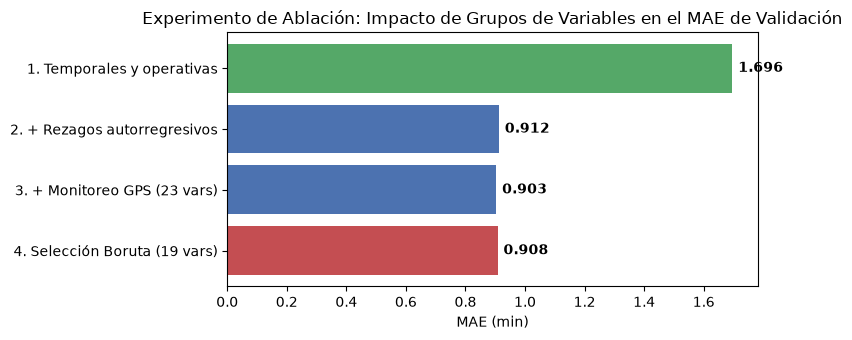
\includegraphics[width=0.82\columnwidth]{figures/ablacion_mae.png}
\caption{Impacto de los subconjuntos de características en el MAE de validación.}
\label{fig:ablation}
\end{figure}

\subsection{Optimización de Hiperparámetros Fuera de Muestra (OOF)}
Sobre Train+Val (5 pliegues expansivos), LightGBM alcanzó un MAE OOF de 0.9029 min frente a 0.9126 min de XGBoost (hiperparámetros óptimos: lr=0.0497, num\_leaves=62, min\_child\_samples=23, n\_estimators=500, reg\_lambda=0.761, subsample=0.828, colsample=0.725). Se seleccionó definitivamente LightGBM por su menor MAE OOF y velocidad.

\subsection{Evaluación Definitiva en el Conjunto de Prueba (Test)}
En el conjunto de prueba independiente ($N=17\,257$ obs, 1\,133 vueltas físicas), evaluado una sola vez con 2\,000 remuestreos bootstrap agrupados por vuelta (Tabla~\ref{tab:test}): LightGBM obtuvo un MAE de 0.840 min [IC 95\,\%: 0.818, 0.862], RMSE de 1.367 min [1.301, 1.439] y $R^2$ de 0.924 [0.913, 0.933]. La reducción pareada de MAE respecto a la persistencia fue de -0.483 min [-0.502, -0.465]. El 91.12\,\% de las predicciones tuvieron un error $\le 2$ min (frente a 86.30\,\% de la persistencia, ganancia neta de +4.82 puntos porcentuales). La prueba pareada de Wilcoxon agrupada por vuelta física ($N=1\,122$ vueltas evaluables) confirmó la superioridad de LightGBM en el 94.30\,\% de los recorridos ($W = 15\,239.0, p = 8.12 \times 10^{-168}$).

\begin{table}[t]
\caption{Evaluación final en Test con IC 95\,\% (Bootstrap de vueltas).}
\label{tab:test}
\centering
\scriptsize
\resizebox{\columnwidth}{!}{
\begin{tabular}{lccc}
\toprule
\textbf{Modelo} & \textbf{MAE (min)} & \textbf{RMSE (min)} & \textbf{\% $\le$2m} \\
\midrule
Persistencia ($last\_known$) & 1.324 & 1.988 & 86.30\,\% \\
\quad \textit{IC 95\,\%} & \textit{[1.294, 1.352]} & \textit{[1.919, 2.068]} & \textit{[85.66, 86.94]} \\
\addlinespace[0.5ex]
LightGBM Final & \textbf{0.840} & \textbf{1.367} & \textbf{91.12\,\%} \\
\quad \textit{IC 95\,\%} & \textit{[0.818, 0.862]} & \textit{[1.301, 1.439]} & \textit{[90.58, 91.64]} \\
\addlinespace[0.5ex]
Mejora neta & \textbf{-0.483} & \textbf{-0.621} & \textbf{+4.82\,\%} \\
\quad \textit{IC 95\,\%} & \textit{[-0.502, -0.465]} & \textit{[-0.672, -0.575]} & \textit{[+3.54, +5.88]} \\
\bottomrule
\end{tabular}
}
\end{table}

\begin{figure}[b]
\centering
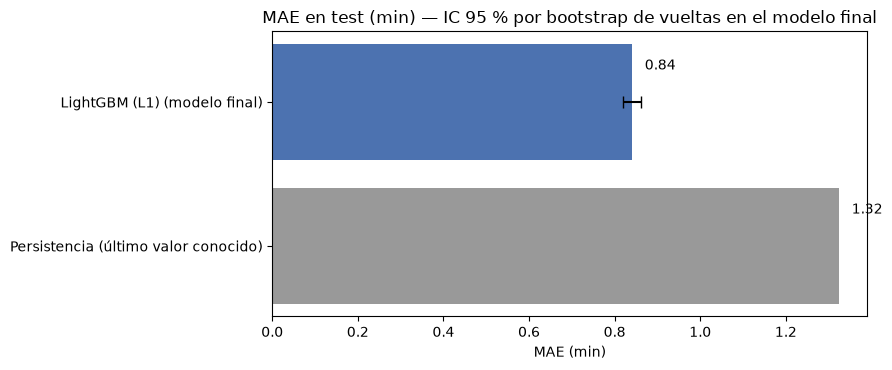
\includegraphics[width=0.82\columnwidth]{figures/test_comparacion.png}
\caption{Comparación de MAE en Test e IC al 95\,\% por bootstrap de vueltas.}
\label{fig:test}
\end{figure}

\subsection{Diagnóstico de Errores e Interpretabilidad SHAP}
El MAE fue de 0.390 min para llegadas en horario ($|d|=0$), ascendiendo a 1.545 min en retrasos severos ($|d| \in [11, 30]$). Sin $lag_1$ disponible (8.2\,\% de casos), el MAE subió a 1.369 min, superando a la persistencia (1.842 min). Por día, el porcentaje $\le 2$ min fue de 93.6\,\% los lunes y 83.1\,\% los sábados.

Los valores TreeSHAP y la importancia por permutación identificaron a \textit{last\_known}, \textit{lag1} y \textit{offset\_min} como los factores que explican más del 70\,\% de la predicción, mostrando efectos monótonos sin artefactos espurios. El clustering $K$-Means ($K=2$, silueta = 0.659) tipificó dos perfiles: vueltas con adelanto severo de madrugada (-9.10 min) y operación regular diurna (+1.61 min).

\section{Discusión Científica y Metodológica}
\textbf{Superioridad del boosting:} Los árboles particionan eficientemente relaciones disyuntivas (uso de \textit{last\_known} cuando $lag_1$ falta), superando la linealidad estricta y evitando la pesada calibración del MLP. Frente a Random Forest, LightGBM requirió 56.5 s en el ajuste de hiperparámetros comparado con 417 s de Random Forest (7.4 veces más lento), manteniendo además una latencia de inferencia de microsegundos indispensable para sistemas embarcados en tiempo real.

\textbf{Monitoreo GPS vs. Rezagos:} El paso por puntos de control fijos ya integra físicamente la velocidad media en el tramo recorrido. La telemetría GPS del tramo cerrado previo $[k-2, k-1]$ sufre de latencia de reporte y vacíos de señal (21.6\,\% de valores faltantes). Aunque su inclusión aporta una modesta reducción de error (-0.009 min de MAE), los rezagos autorregresivos concentran más del 70\,\% del poder explicativo.

\textbf{Resolución y cuantización temporal:} Dado el truncamiento entero de \textit{difference\_time}, se introduce un ruido de cuantización uniforme en $(-1, +1)$ minuto cuya desviación típica teórica es $\sigma \approx 1/\sqrt{12} \approx 0.289$ min. Un MAE de 0.840 min demuestra que el modelo aprende adecuadamente la dinámica macroscópica del retraso, operando en la cercanía de la resolución intrínseca de los registros.

\section{Conclusiones}
Se demostró la viabilidad técnica de predecir la puntualidad del transporte público de Cusco con un error medio de 0.840 minutos [IC 95\,\%: 0.818, 0.862] y el 91.12\,\% de aciertos dentro de $\pm 2$ minutos mediante LightGBM. Se corrigió la pseudoreplicación estadística probando una superioridad en el 94.30\,\% de las vueltas físicas evaluables ($p = 8.12 \times 10^{-168}$). La auditoría semántica (confirmando el truncamiento entero en el 100.0\,\% de observaciones válidas) y el experimento de ablación controlado (46.2\,\% de ganancia por rezagos frente a beneficios marginales de la telemetría previa) constituyen aportes metodológicos reproducibles que desmitifican el uso acrítico de datos GPS sin modelar la inercia autorregresiva.

\section{Limitaciones y Trabajos Futuros}
El horizonte abarca 4 semanas de temporada vacacional sin domingos en test. Como trabajo futuro se propone evaluar la generalización anual en temporada escolar y festividades, así como integrar telemetría de tramo en tiempo real para control preventivo de retención (\textit{holding}) en paraderos.

\begin{thebibliography}{12}
\bibitem{petersen2019} N. C. Petersen, F. Rodrigues, and F. C. Pereira, ``Multi-output bus travel time prediction with convolutional LSTM neural network,'' \emph{Expert Syst. Appl.}, vol. 120, pp. 426--435, 2019.
\bibitem{pang2019} J. Pang, J. Huang, Y. Du, H. Yu, Q. Huang, and B. Yin, ``Learning to predict bus arrival time from heterogeneous measurements via recurrent neural network,'' \emph{IEEE Trans. Intell. Transp. Syst.}, vol. 20, no. 9, pp. 3283--3293, 2019.
\bibitem{liu2020} H. Liu, H. Xu, Y. Yan, Z. Cai, T. Sun, and W. Li, ``Bus arrival time prediction based on LSTM and spatial-temporal feature vector,'' \emph{IEEE Access}, vol. 8, pp. 11917--11929, 2020.
\bibitem{he2020} P. He, G. Jiang, S.-K. Lam, and Y. Sun, ``Learning heterogeneous traffic patterns for travel time prediction of bus journeys,'' \emph{Inf. Sci.}, vol. 512, pp. 1394--1406, 2020.
\bibitem{yu2018} B. Yu, H. Wang, W. Shan, and B. Yao, ``Prediction of bus travel time using random forests based on near neighbors,'' \emph{Comput.-Aided Civ. Infrastruct. Eng.}, vol. 33, no. 4, pp. 333--350, 2018.
\bibitem{ratneswaran2023} S. Ratneswaran and U. Thayasivam, ``An improved bus travel time prediction using multi-model ensemble approach for heterogeneous traffic conditions,'' in \emph{Proc. IEEE ITSC}, 2023, pp. 2410--2415.
\bibitem{kam2024} S.-H. Kam, Y.-W. Chong, N. F. Ibrahim, S.-L. Keoh, S. Phon-Amnuaisuk, and S. K. Abdul Rahim, ``Predicting estimated time of arrival using boosting models,'' in \emph{Proc. 6th IEEE ICAIIC}, 2024, pp. 467--472.
\bibitem{ranjitkar2019} P. Ranjitkar, L.-S. Tey, E. Chakravorty, and K. L. Hurley, ``Bus arrival time modeling based on Auckland data,'' \emph{Transp. Res. Rec.}, vol. 2673, no. 6, pp. 1--9, 2019.
\bibitem{cats2019} O. Cats, ``Determinants of bus riding time deviations: Relationship between driving patterns and transit performance,'' \emph{J. Transp. Eng. Part A: Systems}, vol. 145, no. 1, Art. 04018078, 2019.
\bibitem{rashvand2024} N. Rashvand, S. S. Hosseini, M. Azarbayjani, and H. Tabkhi, ``Real-time bus arrival prediction: A deep learning approach for enhanced urban mobility,'' in \emph{Proc. ICORES}, 2024, pp. 123--132.
\bibitem{cristobal2019} T. Cristóbal, G. Padrón, A. Quesada-Arencibia, F. Alayón, G. De Blasio, and C. R. García, ``Bus travel time prediction model based on profile similarity,'' \emph{Sensors}, vol. 19, no. 13, Art. no. 2869, 2019.
\bibitem{vijaya2024} A. Vijaya, S. Bhattarai, L. S. Angreani, and H. Wicaksono, ``Enhancing transparency in public transportation delay predictions with SHAP and LIME,'' in \emph{Proc. IEEE IEEM}, 2024, pp. 1285--1289.
\end{thebibliography}

\end{document}